\chapter{Theoretical background}
\section{Principles of ecosystem simulation}
\subsection{Ecosystem}
In general we can consider a \emph{System} as any phenomenon that has at least two separable components working together through some interaction. The system can be either structural or functional. Systems can consist of smaller systems, each component being system on their own thus any particular system is part of a hierarchy of other systems. Therefore there is need to define scope and limits in order to not miss any important environmental relationships but on the other hand not to be overwhelmed with irrelevant information. 

Ecological systems are larger systems of nature. That systems can begin with individual organism and expand toward greater complexity such as \emph{communities} or \emph{populations}. Communities, together with non-organic elements form \emph{ecosystems}. The definition is rather arbitrary, and there is no specific way of defining that system. In practice the boundaries are set by investigator, and all interactions and structures within that boundaries form an \emph{ecosystem}. Generally it contains some species like trees or dogs and components of landscape like terrain, lakes or cities. Very large continental-sized ecosystems with strong biotic continuity are called \emph{biomes}. 

Ecosystems are controlled by external and internal factors, such as climate, topography material or cyclic life and competition between species present in that system.
\cite{Hall_Day_1977}

\subsection{Modeling Ecosystem}
\label{modeling_ecosystem}
Model is abstract representation or simplification of an system that is used for studying and simulations. Models are simpler than real systems and have just the most important functional attributes of the real system. Modeling can be used to better understand real ecosystems and aid the conceptualization and measurement of real complex systems. Another use is to predict the consequences of an action that would be expensive, devastating, or difficult to accomplish in the real ecosystem, or just to see "what if". Complexity of nature is often overwhelming, therefore modeling is needed to fully understand it, however models must be checked frequently against real world to ensure that their representation is accurate, at least in areas that we are concerned about.

Two major types of ecological models are \emph{analytic models} and \emph{simulation models}. Both approaches are intended to  increase our understanding and prediction of ecosystems and their components, but in practice the two methods are used for completely different questions. With the analytical model we have more calculations and advanced mathematics, while with the simulation approach we use simpler mathematics, heuristic solutions and greater use of computers.

Analytic models are rather simple, often linear systems, that can be accurately described by a set of mathematical equations whose behavior is well-known. On the other hand, simulation models use numerical computations to solve problems that are impossible or impractical to solve with analytic approach. Simulation models are more widely used, and are generally considered more ecologically realistic, while analytic models are great for their explanatory power and conciseness.

\subsection{Lotka-Volterra equations}
Lotka-Volterra equations are also known as the predator-prey equations. They are a pair of first-order nonlinear differential equations. They are used to describe the dynamics of biological or ecological systems with two interacting species, one as predator and one as prey. The equations contains populations change through time and growth rates of the two populations.

\begin{equation}
    \frac{dx}{dt} = \alpha x - \beta xy,
\end{equation}
\begin{equation}
    \frac{dy}{dt} = \delta xy - \gamma y,
\end{equation}

where
\begin{itemize}
    \item $x$ is the number of prey;
    \item $y$ is the number of predators;
    \item $\frac{dy}{dt}$ and $\frac{dx}{dt}$ represent the instantaneous change rates of the two populations;
    \item $t$ represents time;
    \item $\alpha, \beta, \gamma, \delta$ are positive real parameters describing the interaction of the two species
\end{itemize}

\subsubsection{Lotka-Volterra model limitations}
\label{lotkaVolterraLimitations}
As this model is analytical one, it has its limitations: \cite{lotka_volterra_wiki}
\begin{enumerate}
    \item The prey population is able to find food at all times.
    \item Prey is the only food source for predators.
    \item The rate of change of population is proportional to its size.
    \item During the process, the environment does not change in favour of one species, and genetic adaptation is inconsequential.
    \item Predators and are always willing to eat prey.
\end{enumerate}

\subsubsection{Prey equation explanation}
Term $\alpha x$ represents growth in population. Growth is exponential, as prey has unlimited food supply.
Term $\beta xy$ on the other hand is the rate of predation upon prey. It is proportional to the rate at which they meet, and sizes of both populations, meaning that if either $x$ or $y$ is zero, then there will be no predation.

Interpretation of whole equation: the rate of change in prey's population is equal to its own growth rate minus rate at which it is prayed upon.

\subsubsection{Predator equation explanation}
Term $\delta xy$ represents growth in population, as it is rate of predation (different constant is used, because population growth is not is not necessarily equal to the rate at which prey is eaten).
Term $\gamma y$ corresponds to the loss rate of the predators, due to emigration or natural death of individuals. This leads to exponential decay when there is no pray to supply predators growth.

Interpretation of whole equation: the rate of change in predator's population is determined by rate it consumes prey minus death rate.

\subsubsection{Solutions to the equations}
\begin{figure}[H]
    \centering
    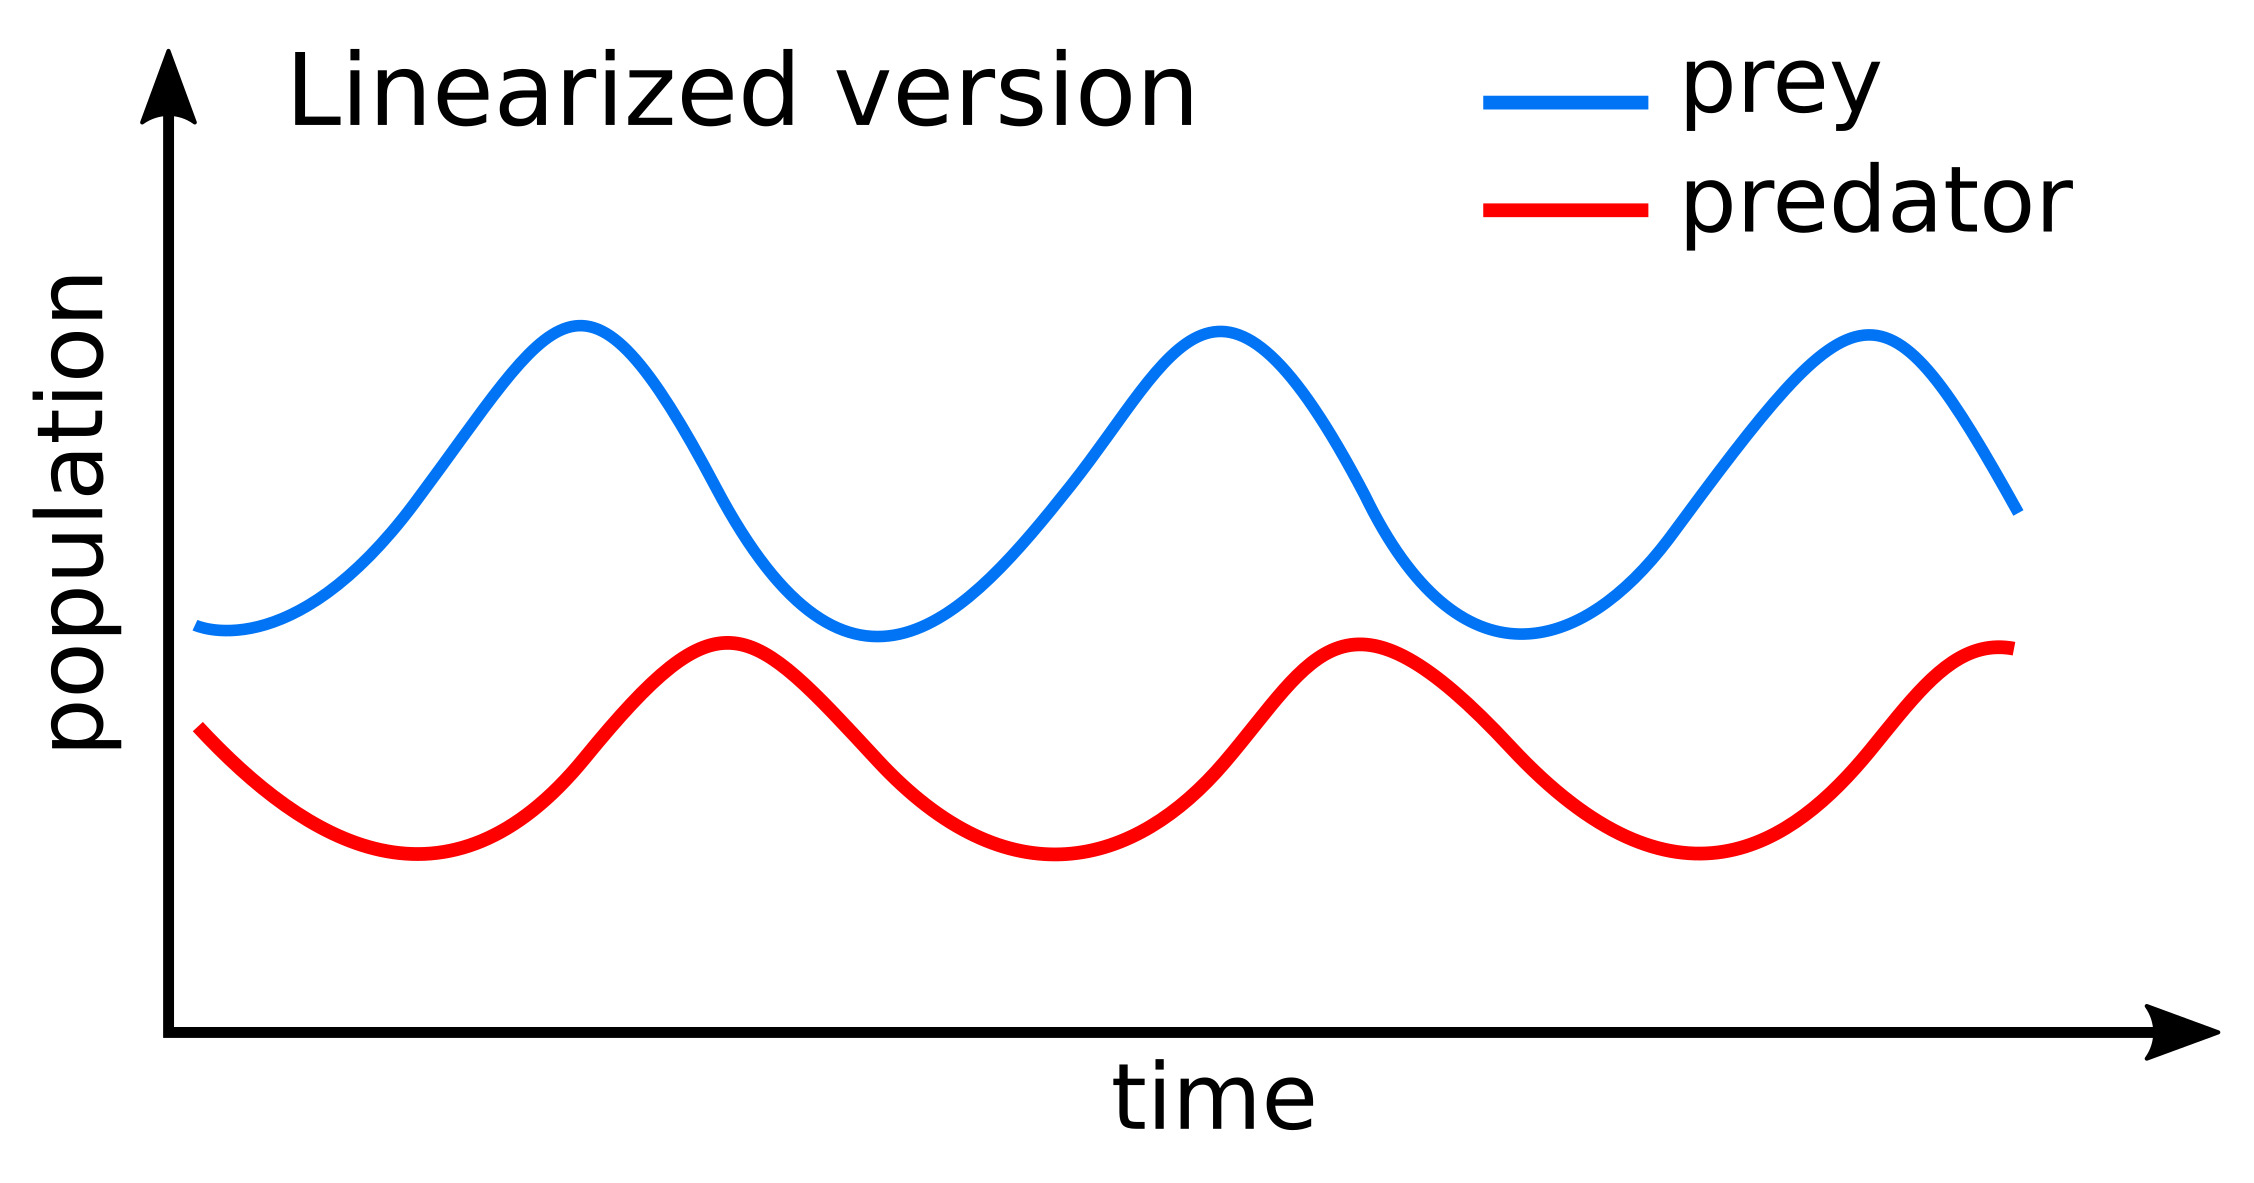
\includegraphics[width=0.6\textwidth]{Images/Lotka_Volterra_dynamics.jpg}
    \caption{Draft of solutions to Lotka-Volterra equations \cite{Lotka_Volterra_dynamics}}
    \label{fig:Lotka_Volterra_dynamics}
\end{figure}

Equations have periodic solutions with the population of predators trailing that of prey by $\pi/2$ in the cycle.
\\
\\
There are generalizations of the Lotka-Volterra equations, such as equations for n species or equations that include competition between those species \cite{BHARGAVA1989319}.

\section{Machine learning}
\emph{Machine Learning} is study of computer algorithms that are able to modify or adapt their actions through experience and use of data, so that these actions become more accurate. Machine learning is part of the broader topic of Artificial Intelligence.

When talking about machine learning it is good to define what learning actually is. The definition of \emph{learning} used in this thesis is getting better at some task through practice. This leads to question: how computer knows if it is getting better at some task. Answering that question provide a way to classify different algorithms int three main types:
\begin{enumerate}
    \item Supervised learning
    \item Unsupervised learning
    \item Reinforcement learning \cite{marsland_2015}
\end{enumerate}

Training using reinforcement learning was used in this thesis, so the focus is only on its description.

\subsection{Reinforcement Learning}
The goal of reinforcement learning is to learn a \emph{policy}. Policy is a mapping from \emph{observations} to \emph{actions}. An observation is what the agent can measure from its environment (all its sensory inputs) and an action is change to the configuration of agent. In other words agent makes decision based on inputs it receives (observations) and does something (actions).

The main element of reinforcement learning is the reward signal. Rewards allow the algorithm to train its policies, as they give feedback on whether the actions taken by the agent were appropriate or not. 

\subsubsection{Training}
Training this model involves taking some initially random action and then, based on the feedback from the reward, adjusting the probability of new actions so that they better fit the goal and receive a larger reward.

\begin{figure}[H]
    \centering
    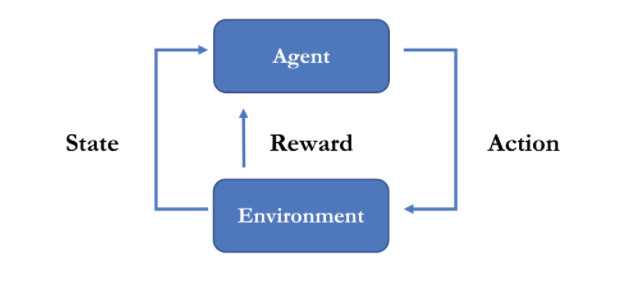
\includegraphics[width=\textwidth]{Images/rl_cycle.jpg}
    \caption{The reinforcement learning cycle. \cite{rlCycle}}
    \label{fig:rlCycle}
\end{figure}

\subsubsection{Curriculum learning}
Curriculum learning is a way of training a machine learning model where more difficult aspects of a problem are gradually introduced in such a way that the model is always optimally challenged.

\subsection{Observations and Sensors}
For an agent to learn, observations should contain all the information the agent needs to perform its task. Without sufficient and relevant information, the agent may learn poorly or may not learn at all. A reasonable approach to determining what information should be included is to consider what would be needed to compute an analytical solution to the problem, or what a human might be expected to be able to use to solve the problem. 

There can be many types of sensors, but the focus here is on two: \emph{vector sensor} and \emph{grid sensor}. A vector sensor is simply a vector of real values that are sent to the policy. The sensor uses a set of box queries in a grid shape and gives a top-down 2D view around the agent. During observations, the sensor detects the presence of detectable objects in each cell and encode that into one-hot representation. The collected information from each cell forms a 3D tensor observation and will be fed into the convolutional neural network of the agent policy (CNNs are a class of artificial neural networks that are most commonly used to analyze visual images). The observation for each grid cell is a one-hot encoding of the detected object. The total size of the created observations is $x_g \times\ y_g \times n$, where $x_g$ and $y_g$ are size of grid in each dimension and $n$ is number of elements that the agent can recognize. \cite{MLAgentsSensors}

\subsubsection{One-hot encoding}

In one-hot encoding, a separate bit of state is used for each state. It is called one-hot because only one bit is “hot” or TRUE at any time. \cite{harrisOneHot}

\subsection{The machine learning process}
There are some common steps for solving given problem using machine learning.
\begin{enumerate}
    \item Data Collection and Preparation
    \item Feature Selection
    \item Algorithm Choice
    \item Parameter and Model Selection
    \item Training
    \item Evaluation \cite{marsland_2015}
\end{enumerate}

\section{Genetic algorithms}
\emph{Genetic} algorithms are metaheuristics inspired by process of natural selection. They are a part of Evolutionary Computation which is one of the three pillars of Computational Intelligence (CI). The CI is the theory, design, application and development of biologically and linguistically motivated computational paradigms. \cite{what_is_ci}
Two other parts are Neural Networks and Fuzzy Systems. CI, and therefore genetic algorithms are used to develop systems, including games, in which agents behave intelligently.

There is no clear definition of genetic algorithms, but most methods that called GAs have following gears in common:
\begin{itemize}
    \item Population of chromosomes
    \item Selection according to fitness
    \item Crossover to produce new offspring
    \item Random mutation of new offspring
\end{itemize}

\subsection{Principles of Genetic Algorithms}
In a genetic algorithm, a population of candidate solutions is evolved toward better solutions (more information on what it means to find a better solution can be found later in this chapter). These solutions are called individuals, creatures or phenotypes. Each candidate has a set of properties, called \emph{genotype} or \emph{chromosomes}, that can be altered or mutated in order to evolve into better solution. There are many ways to represent a chromosome, but one of the most popular representations is a binary string of 0s and 1s. For problems involving numbers, these can be converted to their binary representation so that they can be used in this representation.

The algorithm usually starts with a population of randomly generated individuals. For each iteration, called a generation, fitness is calculated and inferior solutions are replaced by new ones from the best individuals. The new generation is used in the next iteration of the algorithm. In most cases, the algorithm terminates when the maximum number of generations is reached or when a satisfactory fitness level is reached.

\subsection{Fitness function}
The goal of GA used to solve optimization problems is to find a set of parameter values that maximize some specified, often multi-parameter function. This function is called \emph{fitness function}. In other words, the result of this function indicates how suitable a certain set of parameters, or \emph{chromosome}, is for solving a given problem. 

\subsection{Genetic Operators}
There are three common types of operators: selection, crossover, and mutation.
\begin{enumerate}
    \item \emph{\textbf{Selection}} This operator selects chromosomes in the population for reproduction. Chromosomes that has higher fitness are more likeky to be selected to reproduce (possibly several times).
    \item \emph{\textbf{Crossover}} In crossover one or more off-springs are produced using the genetic material of the parents. There are several types of crossover operator such as \emph{One Point Crossover}, \emph{Multi Point Crossover} or \emph{Uniform Crossover}. The simplest and one of the most commonly used is One Point Crossover, where one random crossover point is selected and the tails of the two parents are swapped to produce new offspring.
    \item \emph{\textbf{Mutation}} This operator randomly flips some of the bits in a chromosome. For example, the string 00000100 can be mutated at its second position, giving 01000100. Mutation can occur at each bit position in a string with some, usually very small probability like 0.001).
\end{enumerate}

\subsection{Simple genetic algorithm}
Most GAs (given a clearly defined problem and a bit string representation for candidate solutions) follow the following algorithm \cite{mitchell_1998}:

\begin{enumerate}
    \item Start with a randomly generated population of $n$ $l$-bit chromosomes (candidate solutions to a problem).
    \item Calculate the fitness $f(x)$ of each chromosome $x$ in the population.
    \item Repeat the following steps until $n$ offspring have been created:
    \begin{enumerate}
        \item Select a pair of parent chromosomes from the current population, the probability of selection being an increasing function of fitness. Selection is done "with replacement", meaning that the same chromosome can be selected more than once to become a parent.
        \item With probability $p_c$ (the "crossover probability" or "crossover rate"), cross over the pair at a randomly chosen point (chosen with uniform probability) to form two offspring. If no crossover takes place, form two offspring that are exact copies of their respective parents. (Note that here the crossover rate is defined to be the probability that two parents will cross over in a single point. There are also "multi-point crossover" versions of the GA in which the crossover rate for a pair of parents is the number of points at which a crossover takes place.)
        \item Mutate the two offspring at each locus with probability $p_m$ (the mutation probability or mutation rate), and place the resulting chromosomes in the new population.
        \item If $n$ is odd, one new population member can be discarded at random.
    \end{enumerate}
    \item Replace the current population with the new population.
    \item Go to step 2.


\end{enumerate}